\documentclass[a4paper,12pt]{article}
\usepackage[brazil]{babel}
\usepackage{fancyhdr}  % Pacote para editar cabeçalhos
\usepackage{graphicx}   % Pacote para inserir imagens
\usepackage{amsmath, amssymb}
\usepackage{geometry}
\usepackage{multicol}
\geometry{left=1cm,right=1cm,top=1cm,bottom=1cm}
\usepackage{enumitem}	
\usepackage{titlesec}
\titleformat{\section}{\footnotesize\bfseries}{\thesection}{1em}{}


% Remove a linha preta do cabeçalho
\renewcommand{\headrulewidth}{0pt}  


\pagestyle{fancy}  % Ativa o estilo de cabeçalho
\fancyhf{} % Limpa cabeçalhos e rodapés

% Adiciona as imagens no cabeçalho, ajustando a escala conforme necessário
\fancyhead[L]{\hspace{7cm}\raisebox{-2cm}{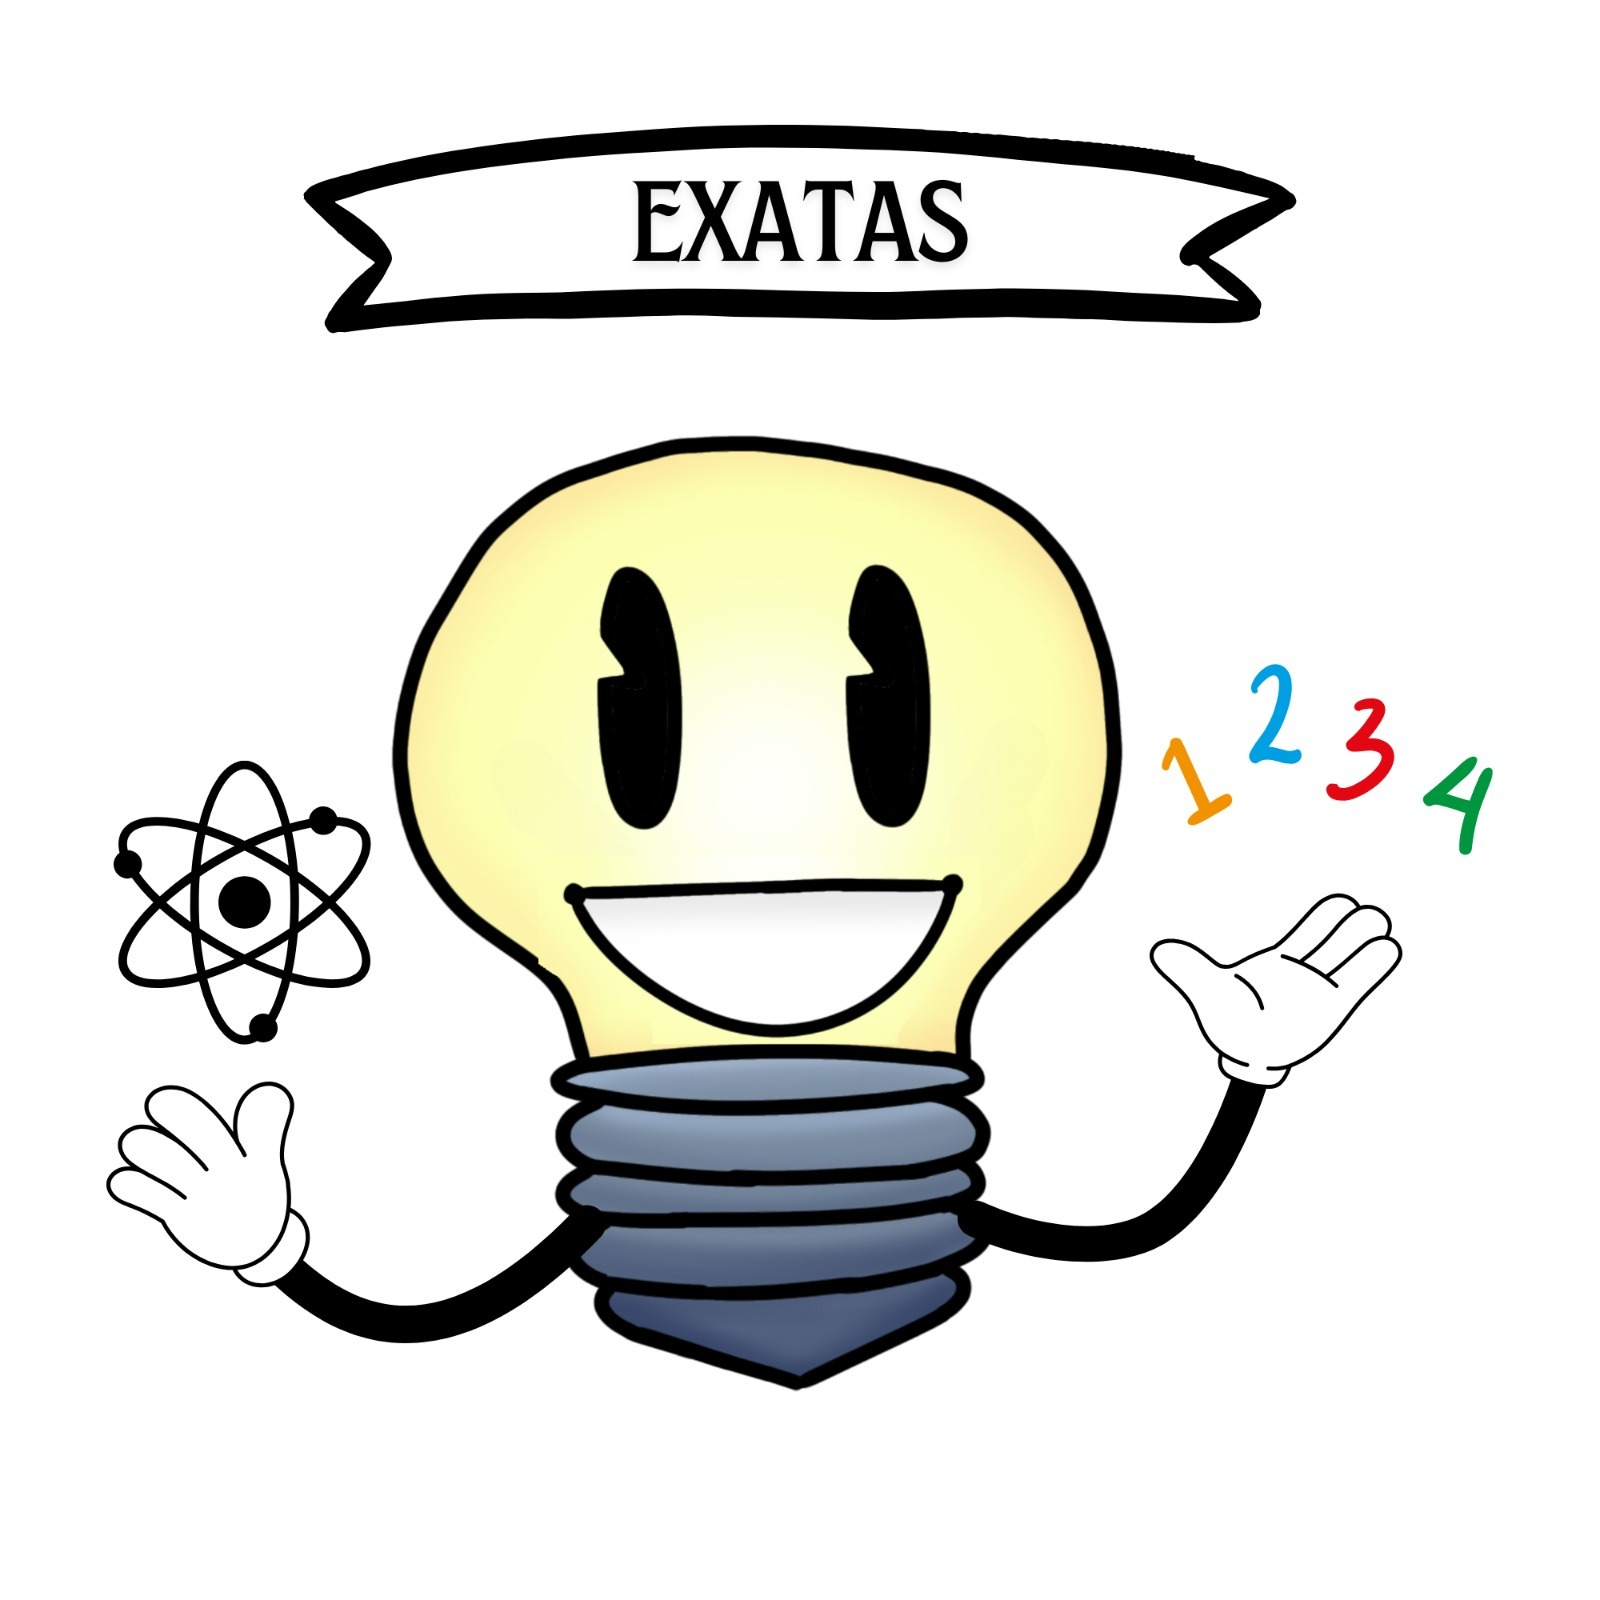
\includegraphics[width=2cm]{exata.jpg}}}  % Esquerda
\fancyhead[R]{\hspace{1cm}\raisebox{-5cm}{
\includegraphics[width=4cm]{pei.jpg}}} % Direita

\begin{document}	
	\begin{multicols}{2}
		
		\section*{Definição de Potenciação} \vspace{-5mm}
		Resolva as expressões abaixo: \vspace{-4mm}
		\begin{multicols}{3}
		\begin{enumerate}[label=\roman*.]
			\item $2^3$ \item  $2.5^2$ \item $(1.2)^4$
			\item $5^4$ \item $0.4^3$ \item $\left(\dfrac{2}{3}\right)^2$
			\item $7^2$ \item $1.1^5$ \item $\left(\dfrac{5}{8}\right)^3$
			\item $10^3$ \item $0.25^2$ \item $\left(\dfrac{4}{9}\right)^4$
			\item $3^5$  \item $\left(\dfrac{7}{5}\right)^2$ \item $0.333\ldots^3$ 
		\end{enumerate}
		\end{multicols}
	
		\section*{Propriedades da Potenciação} \vspace{-5mm}
		Resolva aplicando as propriedades da potenciação: \vspace{-4mm}
		\begin{multicols}{2}
		\begin{enumerate}[label=\roman*.]
			\item $2^3 \times 2^4$
			\item $5^6 \div 5^2$
			\item $(3^2)^3$
			\item $7^5 \times 7^{-3}$
			\item $(2 \times 3)^4$
			\item $ \Bigg[ \bigg( \dfrac{3}{2} \bigg)^{2} \Bigg] ^{3}$
		\end{enumerate}
		\end{multicols}
		
		\section*{Potências de Base 10} \vspace{-5mm}
		Resolva as seguintes expressões: \vspace{-4mm}
		\begin{enumerate}[label=\roman*.]
			\item $10^3$;\quad $10^6$;\quad $10^{-2}$
			\item $5 \times 10^4$;\quad $3,2 \times 10^{-3}$
			\item $4,25 \times 10^{-5}$;\quad $23,06 \times 10^{-3}$
		\end{enumerate}
		
		\section*{Potências de Expoente Negativo}\vspace{-5mm}
		Reescreva as expressões com expoente positivo:\vspace{-4mm}
		\begin{multicols}{2}
		\begin{enumerate}[label=\roman*.]
			\item $2^{-3}$
			\item $5^{-2}$
			\item $10^{-4}$
			\item $\dfrac{1}{3^{-2}}$
			\item $\left(\dfrac{2}{5}\right)^{-3}$
			\item $ \Bigg[ \bigg( \dfrac{3}{2} \bigg)^{-2} \Bigg] ^{-3}$
		\end{enumerate}
		\end{multicols}
		
		\section*{Substituição de Variáveis}\vspace{-5mm}
		\begin{enumerate}
			\item Considere $x = 2^3$, $y = 5^{-2}$ e $z = 10^1$. Substitua e resolva:\vspace{-5mm}
			\begin{multicols}{2}
			\begin{enumerate}[label=\roman*.]
				\item $x + y - z$
				\item $\dfrac{x^2}{z} + y$
				\item $(x \times y)^z$
				\item $(x \times z \times \dfrac{x}{z})$
			\end{enumerate}
			\end{multicols}
			\item Sendo $a=2^{7} \times 3^{8} \times 7$ e $b= 2^{5} \times 3^{6}$, o quociente de $a$ por $b$ é igual a:	\vspace{-4mm}
			% \begin{multicols}{2}	
			%	\begin{enumerate}				
			%		\item 252   \item 126
			%		\item 36 	\item 48
			%	\end{enumerate}
			%\end{multicols}
			\item Qual é o número expresso por $(2^{6} \div 2^{4}) + 2^{2}$\vspace{-4mm}
		%	\begin{multicols}{2}	
		%		\begin{enumerate}				
		%			\item $2^{3}$   \item $2^{0}$
		%			\item $2^{4}$ 	\item $2^{5}$
		%		\end{enumerate}
		%	\end{multicols}
			\item Se $x=3^{6}$ e $y=9^{3}$, podemos afirmar que: \vspace{-5mm}
			\begin{multicols}{2}
				\begin{enumerate}				
					\item $x$ é o dobro de y   \item $x=y$
					\item $x-y=1$	\item $y$ é o triplo de x
				\end{enumerate}
			\end{multicols}
		
		\end{enumerate}
		
		
		\section*{Expressões Numéricas com Potências} \vspace{-5mm}
		Calcule o valor das expressões abaixo: \vspace{-3mm}
		%\begin{multicols}{2}
		\begin{enumerate}
			\item $3^3 + 4^2 - 2^4$
			\item $5^2 - 3^3 + 10^1$
			\item $\left(2^3 + 3^2\right) \times 5^{-1}$
			\item $\dfrac{7^2 - 2^3}{3^2}$
			\item $\left(\dfrac{4^3}{2^2}\right)^2$
			\item $1.2^3 + \left(\dfrac{5}{6}\right)^2 - 0.4^4$
			\item $\dfrac{2.5^2 - 1.1^3}{0.5^2} + \left(\dfrac{3}{4}\right)^3$
			\item $ [ (0,4)^{2} ]^{10} \div [ (0,4)^{9} \times (0,4)^{7} \times 0,4] $
		\end{enumerate}
		
		\section*{Problemas com Potenciação}
		Resolva os problemas abaixo:
		\begin{enumerate}
			\item Um micróbio se divide em duas partes idênticas a cada minuto. Se começarmos com um único micróbio, quantos micróbios teremos após 10 minutos?
			\item Uma cidade tem uma população de $10^5$ habitantes. Se a população dobra a cada 20 anos, quantos habitantes haverá em 60 anos?
			\item Um fio elétrico tem $10^{-3}$ metros de espessura. Quantos fios são necessários para formar 1 metro de espessura?
			\item Um grão de arroz tem aproximadamente $5 \times 10^{-2}$ gramas. Quantos grãos são necessários para formar 1 quilograma?
			\item Uma bactéria se divide a cada $20$ minutos, dobrando sua quantidade. Se inicialmente há $2^3$ 	bactérias (ou seja,$ 8$ bactérias), quantas bactérias haverá após $1$ hora?
			\item Um terreno quadrado tem área de $2^8$
			metros quadrados. Se ele for dividido em pequenos quadrados de área $2^3$
			metros quadrados cada, quantos pequenos quadrados cabem no terreno? Em seguida, expresse o resultado como uma potência de $2$.
			\item Uma população de bactérias cresce seguindo a fórmula 
		$P =	5\times 2^{t/2}$, onde $t$ é o tempo em horas. Se inicialmente $(t=0)$ há 5 bactérias, calcule quantas haverá após $4$ horas e simplifique a expressão usando as regras de potenciação.
		\end{enumerate}		
	\end{multicols}

	\hfill
	 
	5. A massa do Sol é de $1 980 000 000 000 000 000 000 000 000$ toneladas e a massa da Terra é de $5 980 000 000 000 000 000 000 000$ kg
	\begin{enumerate}
		\item[(a)] Escreva em notação científica a massa do Sol e a massa da Terra em quilos
		\item[(b)] Quantas vezes a massa do Sol é maior que a massa da Terra?
	\end{enumerate}
	
	\newpage
	
	\section*{Indicações para estudos}
	
	\begin{enumerate}
		\item \textbf{Canais em Português:}
		\begin{itemize}
			\item Matemática Rio (Rafael Procopio) - @MatematicaRio – Explicações didáticas e divertidas sobre diversos temas de matemática.
			
			\item	Ferretto Matemática - @professorferretto
			– Focado no ensino médio, ENEM e vestibulares.
			
			\item Matemática com Rafa Jesus - Tá Lembrando? - @rafajesus\_talembrando
			 – Aborda desde conteúdos básicos até os mais avançados.
			
		\item 	Vestibulandia - @nerckie
	  – Muito útil para quem quer se aprofundar em matemática para concursos e vestibulares.
			
		\item	Khan Academy Brasil - @khanacademyportugue – Explicações detalhadas com vídeos bem organizados.
			
		\item	Dicasdemat Sandro Curió -
		@sandrocuriodicasdemat
		 – Explicações curtas e diretas sobre diversos tópicos.
		 
		 \item Gis com Giz Matemática - @Giscomgiz – Explicações curtas e diretas sobre diversos tópicos.
			
			\item Toda a Matemática
			- @todaamatematica - A matemática das suas origens às últimas pesquisas.
			
			\item Professora Angela Matemática
			- @professoraangelamatematica
			- é possível aprender matemática e também gostar dela.
			
			\item Professor Dr. Rafael Bastos Mr. Bean da Matemática
			- @mrbeandamatematica
			- Com o Mr Bean da Matemática o aprendizado se torna muito mais fácil. 
			
			\item Estude Matemática
			- @estudematematica - Conteúdo para entusiastas da Matemática...
			
			\item Universo Narrado
			- @UniversoNarrado
			- Narrativas que buscam explorar a beleza do universo por meio da ciência e da literatura.
			
			\item Prof. MURAKAMI - MATEMÁTICA RAPIDOLA
			- @Murakami.
		 - Aprenda em pouco tempo e de forma simples, temas em muitos casos considerados difíceis e tenha uma excelente preparação para as suas provas.
		 
		\end{itemize}
	
			\item \textbf{Canais em Inglês:}
			
			\begin{itemize}
				\item 	3Blue1Brown - @3blue1brown– Explica matemática de forma visual e intuitiva.
				
				\item 	Khan Academy - @khanacademy – Um dos maiores canais educacionais, cobrindo desde matemática básica até cálculo avançado.
				
				\item 	Numberphile  - @numberphile – Explora conceitos matemáticos de forma curiosa e divertida.
				
				\item 	PatrickJMT - @patrickjmt – Explica matemática de forma clara e objetiva.
				
				\item 	Mathologer  - @Mathologer – Aborda matemática avançada com uma pegada histórica e visual.
				
				\item 	Eddie Woo - @misterwootube – Ensina matemática de maneira acessível e envolvente.
							
				
				
			\end{itemize}
			
			\item \textbf{Plataformas e Sites Educacionais:}
			\begin{itemize}
				\item 	Khan Academy – Plataforma gratuita com vídeos, exercícios e acompanhamento de progresso.
				
			\item	Brasil Escola – Explicações teóricas, exercícios e materiais de apoio.
				
		\item		Só Matemática – Exercícios, jogos matemáticos e materiais didáticos.
				
			\item 	Descomplica – Plataforma paga com aulas para ensino médio e vestibulares.
				
		\item		Fuvestibular – Material gratuito para vestibulares e Enem.
			\end{itemize}
		
			
			
			
	\end{enumerate}
	

\end{document}
